\section{Problematiche} \label{sec:prob}
In questa sezione verranno descritti brevemente per chiarezza i problemi che il sistema si propone di risolvere, che sono stati oggetto di studio per lo stagista che ha dovuto analizzarli e cercarne una soluzione.
\subsection{Camera Calibration} \label{sec:camcalib}
Per \textit{camera calibration} si intende la procedura volta a calcolare la relazione matematica tra le coordinate di un punto posizionato nello spazio e la sua proiezione sull'\textit{image plane} di una telecamera. \\

\subsubsection{Intrinsics parameters}
La visione ha origine dall'individuazione della luce nell'ambiente. La luce parte da una qualche sorgente per poi viaggiare nello spazio fino ad incontrare un oggetto, in quel momento buona parte della luce viene assorbita, la parte che non viene assorbita viene riflessa e determina il colore dell'oggetto. \\

Il modello più semplice disponibile per la rappresentazione di una telecamera è il cosiddetto \textit{pinhole camera model}. In tale modello la luce arriva da un oggetto distante, ma solo un singolo raggio entra per ogni particolare punto. Tale punto viene proiettato su di una superficie. Ciò comporta che l'immagine presente sull'\textit{image plane} è sempre a fuoco, e la sua dimensione dipende dalla distanza della sorgente della luce (\textit{focal lenght}).

Si può vedere in figura ~\ref{fig:calib1}) una rappresentazione di tale modello.
\begin{figure}[htpb] 
\centering 
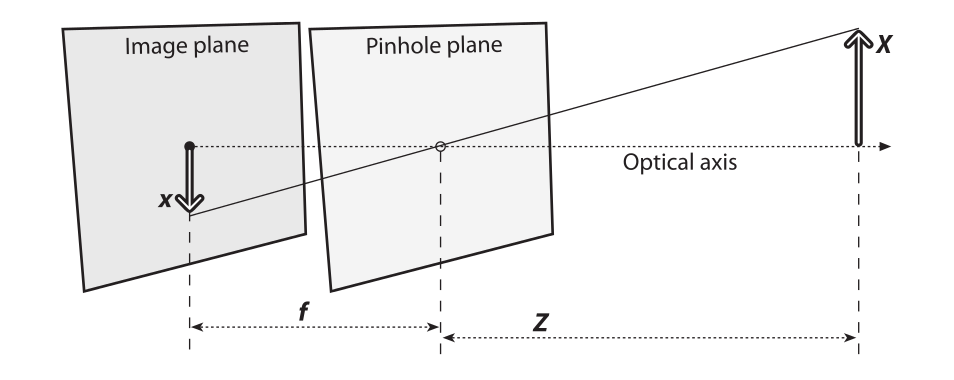
\includegraphics[scale=0.4]{./images/calib1.png} 
\caption{Rappresenzazione di un pinhole camera model} 
\label{fig:calib1}
\end{figure} 

In tale figura \textit{f} è la \textit{focal lenght} della telecamera, \textit{Z} la distanza tra oggetto e telecamera, \textit{X} la dimensione dell'oggetto e \textit{x} l'immagine dell'oggetto proiettata sul piano. \\ Il modello appena descritto può essere reinterpretato come in figura ~\ref{fig:calib2} 
\begin{figure}[htpb] 
\centering 
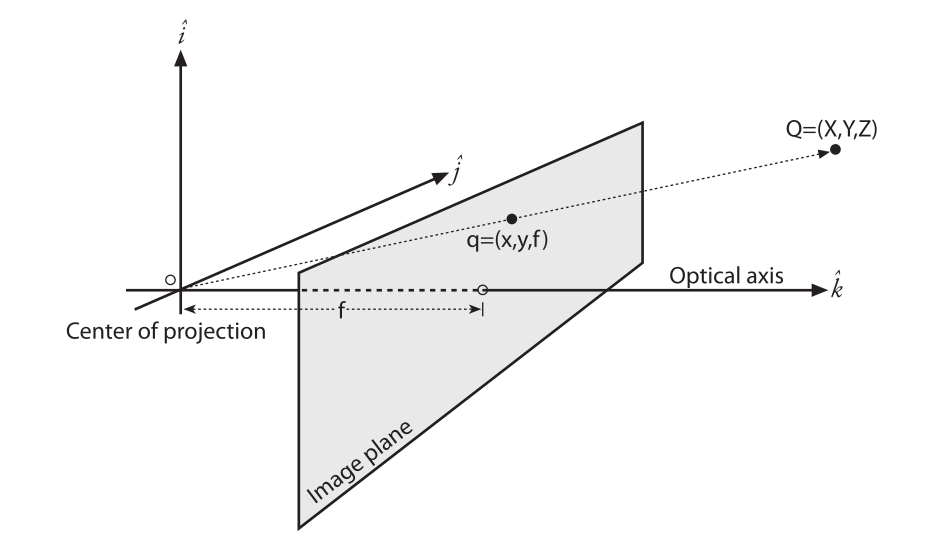
\includegraphics[scale=0.4]{./images/calib2.png} 
\caption{Rappresenzazione di un pinhole camera model rovesciato} 
\label{fig:calib2}
\end{figure} 

nella quale sono stati rovesciati il punto di \textit{pinhole} e l'\textit{image plane}. Ciò ci permette di semplificare le relazioni che valgono tra i punti dell'oggetto e le loro proiezioni. Infatti ora è più chiara la similarità dei 2 triangoli (il primo identificato da \textit{o}, \textit{q} e la proiezione di \textit{q} sull'optical axis e il secondo identificato da \textit{o}, \textit{Q} e la proiezione di \textit{Q} sull'optical axis), inoltre l'immagine non è più capovolta come era in figura ~\ref{fig:calib1}. In tale visione vanno aggiunti altri due nuovi parametri \textit{c\textsubscript{x} }e \textit{c\textsubscript{y}} per considerare un eventuale \textit{displacement} del centro delle coordinate sull'\textit{image plane}, dovuto alla possibilità che il centro del chip (della telecamera) non risieda esattamente sopra l'asse indicato in figura ~\ref{fig:calib2} come \textit{optical axis}. \\ \\
In tale visualizzazione c'è una semplice relazione che mappa i punti \textit{Q\textsubscript{i}} nello spazio (coordinate (\textit{X\textsubscript{i}},\textit{Y\textsubscript{i}},\textit{Z\textsubscript{i}})) nei punti sul piano di proiezione (coordinate (\textit{x\textsubscript{i}},\textit{y\textsubscript{i}})), tale relazione è chiamata \textit{projective transform}. Viene riportata in figura ~\ref{fig:calib3}
\begin{figure}[htpb] 
\centering 
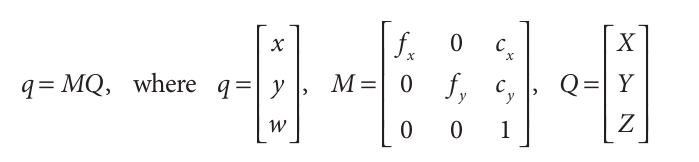
\includegraphics[scale=0.4]{./images/calib3.png} 
\caption{Espressione matematica di una relazione projective transform} 
\label{fig:calib3}
\end{figure} 

Tale modello è utile per capire la meccanica della geometria tridimensionale di visione, ma non è utilizzato nella realtà perche presenta dei limiti. Esso infatti in pratica porterebbe a una frequenza di generazione dei frame molto lenta, dovuta alla bassa quantità di luce che riesce a passare attraverso un \textit{pinhole}. Per ottenere una maggiore quantità di luce e quindi un maggior rapporto di frame/secondo è necessario utilizzare una lente, che consente di raccogliere molta più luce e di curvarla in maniera che converga nel punto di projection. Lo svantaggio di utilizzare una lente è che viene introdotta la \textit{distortion}. \\ \\

\subsubsection{Distortion parameters}

La \textit{lens distortion} si può dividere in due principali tipi:
\begin{enumerate}
	\item \textit{radial distortion}
	\item \textit{tangential distortion}
\end{enumerate}

La prima è un risultato della forma fisica della lente. Le lenti infatti tendono a distorcere i pixel vicini ai bordi dei frame, tale fenomeno è chiamato "barrel effect". Viene riportata in figura ~\ref{fig:calib4} uno schema che aiuta l'intuizione del motivo per cui tale fenomeno si verifica.
\begin{figure}[htpb] 
\centering 
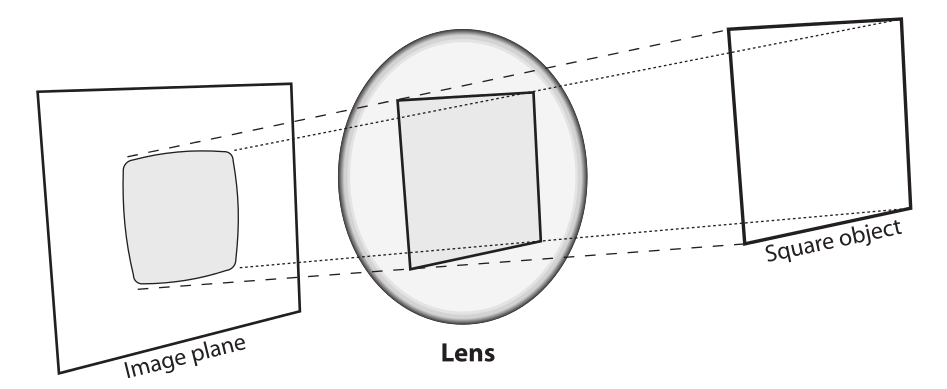
\includegraphics[scale=0.3]{./images/calib4.png} 
\caption{Radial distortion effect} 
\label{fig:calib4}
\end{figure} 
\\ \\
La seconda è un risultato dei difetti di assemblaggio che portano la lente a non essere perfettamente parallela all'\textit{image plane}. Si riporta un immagine che evidenzia tale fenomeno in figura ~\ref{fig:calib5}.
\begin{figure}[htpb] 
\centering 
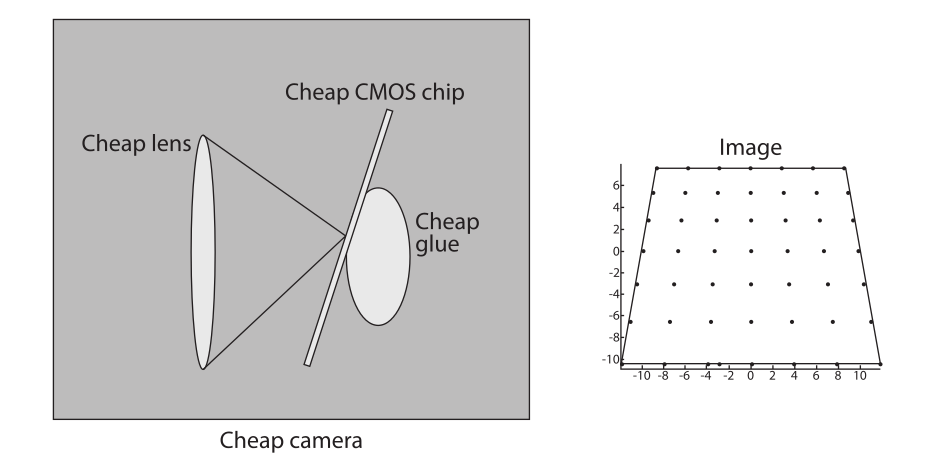
\includegraphics[scale=0.3]{./images/calib5.png} 
\caption{Tangential distortion effect} 
\label{fig:calib5}
\end{figure} 

\subsubsection{Calibrazione}

Ora che è stato descritto come identificare a livello matematico le proprietà \textit{intrinsics} e \textit{distortion} possiamo vedere le tecniche con le quali si prendono in considerazione tali parametri per correggere i frame catturati dalla telecamera.\\
Le tecniche di calibrazione si basano sul seguente criterio: viene mostrato alla camera un oggetto di cui si conosce la struttura, e si valutano le differenze tra le caratteristiche dell'oggetto catturato dalla camera (quindi proiettato sull'\textit{image plane}) con le sue note caratteristiche fisiche. \\Per ogni immagine che una telecamera cattura di un oggetto, è possibile descrivere la sua posizione rispetto al sistema di coordinate della telecamera in termini di rotazione e traslazione. Possiamo quindi definire una relazione tra la posizione nello spazio di un oggetto e le sue coordinate nel frame catturato dalla telecamera. Combinando tale relazione con le correzioni derivanti dai parametri di \textit{intrinsics} si ottiene un sistema di equazioni che risolto rappresenta la soluzione al problema della calibrazione.\\
In linea di principio qualsiasi oggetto può essere usato ai fini di tale operazione, ma è pratico utilizzare un oggetto che presenta caratteristiche regolari (pattern). All'interno del progetto è stata  utilizzata una immagine di una scacchiera con dimensioni (numero di celle) predefinite.  \\
Si potrà vedere come OpenCV offre un API di alto livello per la soluzione del problema della calibrazione con l'utilizzo di una scacchiera.

\subsection{Tracking data transformation}

Il sistema di \textit{video analytics} utilizza le funzionalità offerte da OpenCV per tracciare i movimenti delle persone. Non scenderemo nei dettagli di come ciò viene effettivamente implementato, basti sapere che il sistema è in grado di tracciare diversi oggetti contemporaneamente. Si riporta uno screenshot che mostra il risultato di tale operazione in figura ~\ref{fig:track1}.
\begin{figure}[htpb] 
\centering 
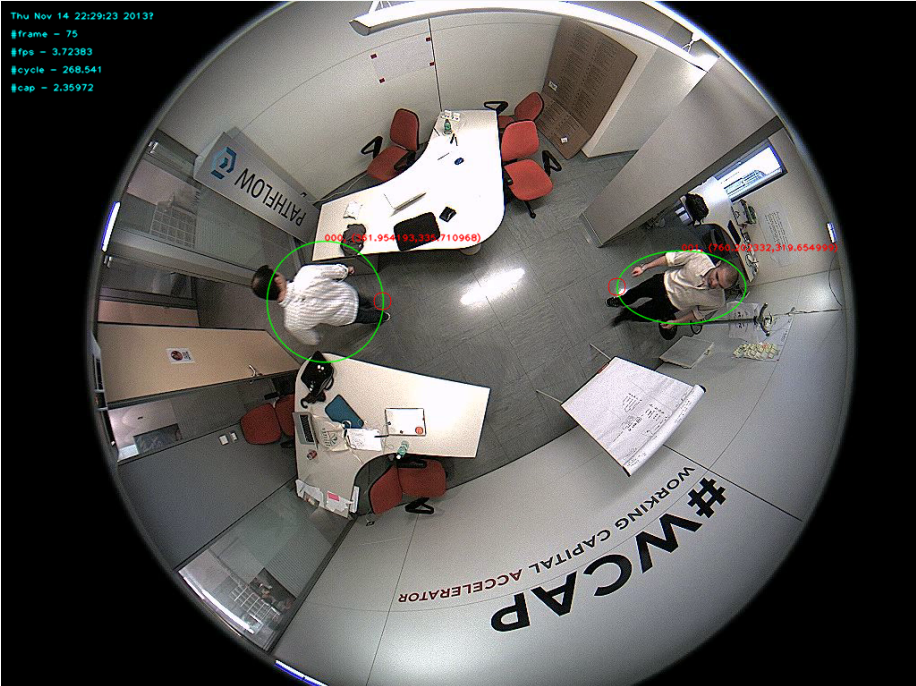
\includegraphics[scale=0.4]{./images/track1.png} 
\caption{Screenshot preso dallo stream video della camera che mostra come gli oggetti vengono tracciati} 
\label{fig:track1}
\end{figure} 
 L'output di tale processo consiste di un timestamp e delle coordinate (\textit{x} e \textit{y}) che esprimono la posizione dell'oggetto all'interno del frame della telecamera. Il sistema di coordinate che OpenCV utilizza per esprimere tali posizioni considera la posizione dell'origine in basso a sinistra del frame, ed ovviamente si basa su interi in quanto considera come unità sugli assi il pixel (ogni pixel nel frame indica una posizione).
Tali dati contengono le informazioni di tracciamento ma non sono direttamente utilizzabili in quanto il tipo di elaborazione che il progetto si propone di fare si basa su delle coordinate che non sono relative ad un particolare frame ma che sono relative ad una piantina (planimetria) del locale dove sono presenti le telecamere. Per questo è necessario che tali dati (che chiameremo \textit{raw}) vengano trattati per essere trasformati in dati che contengono l'informazione pulita e utilizzabile. Per ottenere tutto ciò è necessario avvalersi di una matrice di trasformazione (\textit{homography matrix}).
\subsubsection{Homography matrix}

Nella \textit{computer vision} viene definita come \textit{planar homography} una relazione che esprime una mappatura da un piano ad un altro. Tale relazione può essere espressa da una matrice (solitamente indicata con \textit{H}), la quale applicata ad un vettore che esprime una posizione nel piano di partenza dà come risultato una posizione nel piano di arrivo. Per calcolare tale matrice è sufficiente avere 4 punti sul piano di partenza e le loro corrispettive coordinate sul piano di arrivo. In figura ~\ref{fig:track2} si riporta una rappresentazione grafica di tale situazione.
\begin{figure}[htpb] 
\centering 
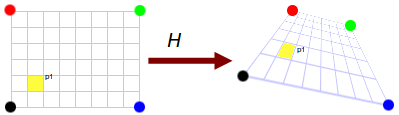
\includegraphics[scale=1.0]{./images/track2.png} 
\caption{I 4 punti necessari per il calcolo della homography matrix} 
\label{fig:track2}
\end{figure} 

Una volta che si hanno a disposizione i punti sui due piani ci sono degli algoritmi noti per calcolare la soluzione del sistema (la matrice). Una volta ottenuta la \textit{homography matrix} è facile anche effettuare l'operazione inversa: la conversione di un punto sul piano di arrivo nel suo corrispettivo nel piano di partenza. L'applicazione della matrice ad un punto per ottenere il suo corrispettivo nell'altro piano si chiama \textit{perspective transformation}. \\
Gli utilizzi delle \textit{homograpy matrices} non si limitano a quanto è stato qui esposto, ma non indagheremo sulle loro diverse applicazioni, basti sapere che quanto è stato utilizzato nel progetto è solo una minima parte dei possibili significati e usi di tali matrici. \\ \\
Nell'implementazione del sistema è stato definito come piano di partenza il "pavimento" del locale dal punto di vista della telecamera, e come piano di arrivo la planimetria del locale. Una volta calcolata la relazione tra i due piani essa verrà utilizzata per trasformare i dati \textit{raw} che escono in output dal processo di tracking in dati puliti (relativi alla planimetria del locale).
Vedremo che OpenCV offre delle funzioni di alto livello per effettuare tale operazione.

\subsection{Qt drawings}
Qt offre molte facilitazioni per eseguire manipolazioni grafiche. All'interno del progetto è stato necessario prima di tutto convertire un immagine contenuta in un file .DXF in un immagine .PNG. Per fare ciò si sono importate alcuni degli elementi presenti nell'immagine vettoriale (i più importanti) e si sono convertiti in elementi \textbf{disegnabili} (per i quali era presente una funzione che permettesse la loro fedele rappresentazione) dalle classi di Qt. Per fare ciò lo stagista ha dovuto tenere conto delle differenze tra il sistema di coordinate utilizzato in un file .DXF e la loro rappresentazione in un sistema Qt-style. Infatti all'interno delle librerie Qt (in particolare ci riferiamo alla classe QPainter che è stata effettivamente utilizzata per disegnare) il sistema di coordinate non è standard (con origine in basso a sinistra) ma è rovesciato specularmente rispetto all'asse x. Ciò ha comportato un ulteriore passaggio. Si riporta in figura ~\ref {fig:qtgrad1} un'immagine chiarificatrice di tale situazione.


\begin{figure}[htpb] 
\centering 
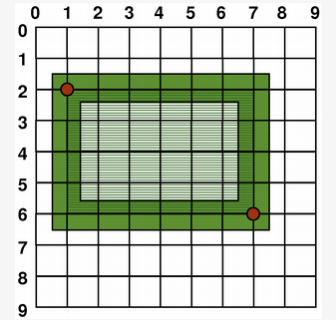
\includegraphics[scale=0.5]{./images/qtgrad1.png} 
\caption{Sistema di coordinate utilizzato per il disegno su Qt} 
\label{fig:qtgrad1}
\end{figure} 

Tale complicazione è sorta anche nell'interpretazione dei dati in output dal sistema di \textit{video analytics} utilizzati per il disegno dell'\textit{heatmap}. Tali dati (come per gli elementi nel file .DXF) utilizzano un sistema di coordinate standard (origine in basso a sinistra). E' quindi stato necessario tenere conto di tale diversità per produrre un risultato coerente.  \\ \\
Per il disegno dell'\textit{heatmap} è stato necessario l'utilizzo di \textbf{gradienti di colore}. Nella computer graphics un gradiente è una struttura che definisce una regione la cui colorazione dipende dalla posizione relativa alla "zona" coperta dal gradiente. 
Per il disegno di una mappa di calore i gradienti utilizzati sono di tipo \textit{radial}: essi sono definiti come delle zone circolari che hanno un determinato colore nel loro centro e un diverso colore ai bordi. Il colore effettivo dei punti interni è calcolato in base alla distanza dal centro del cerchio. \\
Fortunatamente Qt mette a disposizione la classe QGradient (e  derivate) che implementano il \textit{fillings} di particolari zone con gradienti.

